% !TeX spellcheck = el_GR-en_US
\documentclass[11pt]{article}
\usepackage{geometry}
\geometry{a4paper, top=2cm, bottom=2cm, left=2cm, right=2cm}
\usepackage{fontspec}
\usepackage{titlesec}
\usepackage{titling}
\usepackage{float}
\usepackage{subcaption}
\usepackage[nonumeralsign]{xgreek}
\usepackage{fancyhdr}
\usepackage{hyperref}
\usepackage{enumitem}
\usepackage{cite}
\usepackage{multirow}
\usepackage{graphicx}
\usepackage[normalem]{ulem}
\usepackage{float}
\restylefloat{table}
\useunder{\uline}{\ul}{}
\usepackage{amsmath}
\usepackage{cleveref}
\usepackage{booktabs}

\crefformat{footnote}{#2\footnotemark[#1]#3}

\setmainfont{Lato}
\setmonofont{Consolas}

\title{Τεχνολογία Ήχου και Εικόνας 2018\\
    Εργασία 2018-2019}
\author{Χριστίνα Θεοδωρίδου - 8055\\
    Φρανκ Μπλάννινγκ - 6698\\
    Αποστόλης Φανάκης - 8261}
\date{\today}

\pagestyle{fancy}
\lhead{Τεχνολογία Ήχου και Εικόνας 2018}
\rhead{~σ}
\renewcommand{\headrulewidth}{0.4pt}
\renewcommand{\footrulewidth}{0.4pt}
\setlength{\headheight}{14pt}

\hypersetup{colorlinks=true, linkcolor=black, urlcolor=blue, citecolor=blue}
\urlstyle{same}

\begin{document}
    \maketitle
    \tableofcontents
    \newpage

    \section{Εισαγωγή}

Το ζητούμενο της εργασίας είναι η ανάπτυξη ενός μοντέλου μηχανικής
μάθησης το οποίο, παρέχοντας ένα αρχείο ήχου, θα μπορεί να ξεχωρίσει
ανάμεσα στα κομμάτια του χρόνου που περιέχουν ομιλία (speech) και
μουσική (music), όπως παρουσιάζεται στον διαγωνισμό MIREX 2018:Music and/or Speech Detection 
\footnote{https://www.music-ir.org/mirex/wiki/2018:Music\_and/or\_Speech\_Detection} .
Η εργασία επικεντρώνεται στην εύρεση των δειγμάτων που περιέχουν είτε ομιλία είτε μουσική
και στην ταξινόμησή τους.

Πρόκειται για ένα δυαδικό πρόβλημα ταξινόμησης που είναι σημαντικό καθώς έχει
εφαρμογές σε πλατφόρμες κοινωνικών δικτύων για την αναγνώριση
περιεχομένου με πνευματικά δικαιώματά, σε συστήματα αυτόματης
αναγνώρισης διαφημίσεων, μοντέρνα "έξυπνα" βοηθητικά ακοής κ.α. Η
πρόσφατη βιβλιογραφία περιέχει θεματολογία όπου στοχεύει είτε στην
ανάπτυξή αλγορίθμων για γρήγορη και φθηνή υπολογιστικά ταξινόμηση,
είτε στην αναγνώριση πολύ μεγάλης ακρίβειας. Αυτό διότι αυτή τη
στιγμή η αναγνώριση με ποσοστό επιτυχίας γύρω στο 98\% είναι κάτι
συνηθισμένο.
    \section{Προηγούμενες υλοποιήσεις}

Υπάρχει πληθώρα βιβλιογραφίας σχετική με το θέμα. Έχουν βρεθεί ήδη
αρκετές λύσεις, ενώ οι πιο πρόσφατες πετυχαίνουν αξιοσημείωτα
αποτελέσματα τόσο όσων αφορά την ταχύτητα του διαχωρισμού όσο και την ακρίβεια
των αποτελεσμάτων. Κάποιες από τις δημοσιεύσεις οι οποίες αφορούν το
συγκεκριμένο θέμα, καθώς και τα αποτελέσματά τους παρουσιάζονται παρακάτω.

\vspace{1em}
Στο ~\cite{robust} οι συγγραφείς χρησιμοποιούν τα εξής χαρακτηριστικά (features):
\begin{enumerate}[noitemsep]
\item Διαμόρφωση ενέργειας στα 4Hz του σήματος (4Hz modulation)
\item Διαμόρφωση εντροπίας του σήματος (entropy modulation)
\item Αριθμός των στατικών τμημάτων
\item Διάρκεια των τμημάτων
\end{enumerate}

Παρατηρήθηκε πειραματικά ότι τα πρώτα 3 χαρακτηριστικά δίνουν ξεχωριστά περίπου
το ίδιο ποσοστό επιτυχών ταξινομήσεων (περίπου 84\%) ενώ η Μπαγιεσιανή προσέγγιση
για το χαρακτηριστικό δίαρκειας τμημάτων έδωσε λίγο χαμηλότερο ποσοστό (76.1\%). 

Για να αυξηθεί το ποσοστό των συνολικών επιτυχών ταξινομήσεων προτάθηκε ένας
ιεραρχικός αλγόριθμος ταξινόμησης στον οποίο τα χαρακτηριστικά διαμόρφωσης
ενέργειας του σήματος στα 4Ηz και διαμόρφωσης εντροπίας του σήματος συγχωνεύονται.
Σε περίπτωση που οι 2 ταξινομητές συμφωνούν αποφασίζουν για το αν το τμήμα
αποτελεί ομιλία ή όχι, ενώ σε περίπτωση που δεν συμφωνούν, η απόφαση
οριστικοποιείται από το χαρακτηριστικό του αριθμού τμημάτων. Αποδεικνύεται ότι
τα αποτελέσματα αυτού του αλγορίθμου δίνουν 90.1\% σωστές ταξινομήσεις.

\vspace{1em}
Στο ~\cite{mirex} το πρόβλημα που δόθηκε αντιμετωπίζεται ως 2 υποπροβλήματα:
το πρόβλημα εντοπισμού δειγμάτων και το πρόβλημα κατηγοριοποίησής τους.
Για τον εντοπισμό δειγμάτων μουσικής/φωνής εφαρμόστηκε ο αλγόριθμος Random
Forest σε 2 εκδοχές του: στην πρώτη, εφαρμόστηκε μαζί με έναν Silence detection
αλγόριθμο ενώ στη δεύτερη βασίστηκε μόνο στις πληροφορίες ομοιογένειας (self
similarity matrix) και στην λειτουργία του ίδιου του ταξινομητή. Επίσης, για την
ταξινόμηση προτάθηκαν 2 εναλλακτικές: στην πρώτη χρησιμοποιήθηκε ένα
προ-εκπαιδευμένο μοντέλο ενώ στην δεύτερη η εκπαίδευση γίνεται κατά την
αξιολόγηση των δειγμάτων.

Χρησιμοποιήθηκαν τα χαρακτηριστικά (features):
\begin{enumerate}[noitemsep]
\item RMS ενέργεια
\item ZCR (Zero-Crossing Rate)
\item Spectral rolloff (Συχνότητα Αποκοπής)
\item Spectral flux (Φασματική Ροή)
\item Spectral flatness (Φασματική Επιπεδότητα)
\item Spectral flatness per Band (Φασματική Επιπεδότητα ανά συχνοτικές ομάδες)
\item MFCCs (Mel Frequency Cepstral Coefficients)
\end{enumerate}

% TODO: η παράγραφος δε βγάζει και πολύ νόημα μετά από ένα σημείο
Έγινε ανάλυση κύριων συνιστωσών (Principal component analysis ή PCA) με στόχο να
μειωθούν οι διαστάσεις των διανυσμάτων των χαρακτηριστικών (feature vectors).
Δημιουργήθηκαν οι πίνακες ομοιότητας υπολογίζοντας την ευκλείδεια απόσταση
μεταξύ των δειγμάτων ήχου έτσι ώστε να χωριστούν σε τμήματα. Στη συνέχεια τα
τμήματα αυτά κατηγοριοποιούνται ενώ ταυτόχρονα εφαρμόζεται ο αλγόριθμος Silence
Detection. Για το πρόβλημα της
κατηγοριοποίησης χρησιμοποιείται ο ίδιος αλγόριθμος Random Forest για
ταξινόμηση σε επίπεδο τμημάτων ήχου (frame). Εφόσον για κάθε αρχείο ήχου έχουν
εξαχθεί τα παραπάνω χαρακτηριστικά, κάθε τμήμα ήχου ταξινομείται στην κλάση που
αποφασίζεται και έπειτα ολόκληρο το αρχείο ταξινομείται στην κλάση στην οποία
ταξινομήθηκαν τα περισσότερα τμήματά του.

\vspace{1em}
Στο ~\cite{speech} προτείνεται πως τα χαρακτηριστικά μπορεί να μην καλύπτουν
χαρακτηριστικά και της ομιλίας και της μουσικής, αλλά να βασίζονται κυρίως σε
χαρακτηριστικά ενός από τα δύο. Ενδιαφέρον παρουσιάζουν τα χαρακτηριστικά της
ομιλίας, τα οποία λόγω των μέσων που την παράγουν (τα χείλη, η γλώσσα και οι
φωνητικές χορδές) έχουν ιδιαίτερα γνωρίσματα. Η μελέτη αυτών των χαρακτηριστικών
και η χρήση τους σε έναν ταξινομητή αποδεικνύεται πως μπορεί να
αυξήσει την επιτυχία του διαχωρισμού.

Ενδεικτικά, πέρα από το καθιερωμένο χαρακτηριστικό της διαμόρφωσης ενέργειας στα 4Hz (4Hz modulation energy), λόγω του
ρυθμού των συλλαβών, κάποια άλλα χαρακτηριστικά ειδικά για ομιλία βασίζονται στην
αναγνώριση του ήχου που παράγεται στις φωνητικές χορδές κατά την εναλλαγή της
προφοράς ενός συμφώνου σε ένα φωνήεν ή στην μελέτη της αυτοσυσχέτησης του
σήματος μετά από φιλτράρισμα (Zero Frequency Filtered Signal).

\vspace{1em}
Πέρα από την επιλογή των χαρακτηριστικών, η μέθοδος εκπαίδευσης έχει μεγάλη επίπτωση στην
τελική αποτελεσματικότητα του αλγορίθμου. Μερικές φορές χρήση σύνθετων μεθόδων
εκπαίδευσης μπορούν να επιφέρουν καλύτερα αποτελέσματα σε μεγαλύτερο ποσοστό
διότι επιτρέπουν την έξοδο από τοπικά ελάχιστα. Η σύνθετες μέθοδοι μπορεί να μην
είναι συμβατικές ή και να δανείζονται από παρατηρήσεις της φύσης, όπως ο
συνδυασμός ενός Support Vector Machine (SVM) με τον Cuckoo Algorithm ~\cite{cuckoo},
όπου, όπως το πουλί κούκος που γεννάει τα αυγά του σε ξένες φωλιές, στις
επαναλήψεις εκπαίδευσης του SVM κάποιες λύσεις πετιούνται και αντικαθίστανται από
νέες οι οποίες μπορεί να επιφέρουν καλύτερα αποτελέσματα.

\vspace{1em}
Στο ~\cite{hybrid} οι συγγραφείς χρησιμοποιούν τα χαρακτηριστικά:
\begin{enumerate}[noitemsep]
\item ΜFCCs (Mel Frequency Cepstral Coefficients)
\item ZCR (Zero-Crossing Rate)
\item SC (Spectral Centroid)
\item SR (Spectral Rolloff)
\item SF (Specral Flux)
\end{enumerate}

Τα χαρακτηριστικά ΜFCC, ZCR και SF ταξινομούν με ακρίβεια ~90\% το καθένα. Το SR με 83\%, ενώ το SC με 70\%. Ο συνδυασμός όλων των παραπάνω χαρακτηριστικών πετυχαίνει
93.5\% σωστή ταξινόμηση, ενώ με χρήση ενός SVM μοντέλου το ποσοστό φτάνει στο
95.68\%.

Παρατηρείται ότι η σωστή ταξινόμηση της μουσικής είναι αρκετά δυσκολότερη (με
τα συγκεκριμένα χαρακτηριστικά) σε σχέση με αυτή της ομιλίας. Ειδικότερα στην ομιλία
επιτυγχάνεται (με το SVM) ακρίβεια 98.25\% ενώ στη μουσική 93.1\%.

\vspace{1em}
Τέλος, σύμφωνα με το ~\cite{radio}, σε εφαρμογές κατηγοριοποίησης όπου δεν
επιβάλλεται η λειτουργία σε πραγματικό χρόνο, η χρήση χαρακτηριστικών ενέργειας είναι
επιθυμητή λόγω της μεγάλης ακρίβειας τους. Συγκεκριμένα η αναζήτηση της ελάχιστης πυκνότητας ενέργειας (Minimum
Energy Density) δείχνει να υπερέχει από άλλα χαρακτηριστικά ενέργειας τόσο στην
αποτελεσματικότητα της όσο και στην απλότητα του υπολογισμού της. Σε συνδυασμό με το
χαρακτηριστικό της διαφοράς ενέργειάς στα διάφορα κανάλια μιας πολυκάναλης
εισόδου, στο ~\cite{radio} πέτυχαν ακρίβεια 100\% στα κομμάτια εισόδου όπου
περιείχαν μόνο μουσική ή ομιλία και όχι τον συνδυασμό τους (όπως στις ραδιοφωνικές
διατιμήσεις).

    % \section{Σχεδιασμός υλοποίησης}

Μετά από μελέτη των προηγούμενων υλοποιήσεων και πειραματισμό με την εξαγωγή
διάφορων χαρακτηριστικών (features) στη Matlab αποφασίσαμε να ακολουθήσουμε την
παρακάτω πορεία αντιμετώπισης του προβλήματος.

\subsection{Παραθυροποίηση}

Για την παραθυροποίηση του σήματος θα γίνει χρήση Hamming παραθύρων με επικάλυψη
50\%. Η τελική χρονική διάρκεια των παραθύρων αναμένεται να είναι στο πεδίο του
μισού με ενός δευτερολέπτου (0.5-1 sec) και θα καθοριστεί στη πορεία μέσω trial
and error τεχνικών.

\subsection{Χαρακτηριστικά}

Τα χαρακτηριστικά που έχουν επιλεγεί είναι τα εξής:
\begin{enumerate}[noitemsep]
\item ΜFCCs (Mel Frequency Cepstral Coefficients)
\item Silence ratio
\item ZCR (Zero-Crossing Rate)
\item SC (Spectral Centroid)
\item SR (Spectral Rolloff)
\item SF (Specral Flux)
\item 4Hz modulation
\item Minimum Energy Density (MED)
\end{enumerate}

Τα συγκεκριμένα χαρακτηριστικά εμφανίζουν τις μεγαλύτερες ακρίβειες στη
ταξινόμηση ενώ ταυτόχρονα έχουν μικρή ετεροσυσχέτιση. Άλλα χαρακτηριστικά μπορεί
να προστεθούν στη πορεία μετά από αναλυτικότερη έρευνα της βιβλιογραφίας.

\subsection{Μοντέλο ταξινόμησης}

Από την βιβλιογραφική έρευνα διαπιστώθηκε ότι οι διαφορετικές επιλογές
χαρακτηριστικών επηρεάζουν την ακρίβεια των μοντέλων. Έτσι με μία συγκεκριμένη
επιλογή χαρακτηριστικών μπορεί τα πιθανοτικά μοντέλα (Naive Bayes, GMM, κ.α.) να
είναι αποτελεσματικότερα των SVM ή των νευρωνικών. Αλλά με επιλογή διαφορετικών
features να ισχύει το αντίθετο. Για τον λόγο αυτό είναι απαραίτητο, αφού
αποφασιστεί το σετ των χαρακτηριστικών να γίνει εκπαίδευση και testing πολλών
μοντέλων πριν την τελική επιλογή.
Έτσι η πρόταση μας είναι η δοκιμή των περισσότερων ευραίως διαδεδομένων μοντέλων,
όπως: Decision trees, Bayesian networks, Gaussian mixture model, Hidden Markov
Model, SVMs, Artificial Neural networks, Genetic Algorithms.

\subsection{Preprocessing, άλλες τεχνικές}

Περισσότερες και πιο εξεζητημένες τεχνικές θα χρησιμοποιηθούν στο πρακτικό
κομμάτι που θα υλοποιηθεί αργότερα. Κατά το preprocessing των δεδομένων μέθοδοι
όπως data rescaling, data standardization, data binarization, data cleaning,
data integration, data transformation ενδέχεται να φανούν χρήσιμες. Ακόμα, κατά
την εκπαίδευση διάφορες γνωστοί μέθοδοι validation όπως το k-fold cross-validation,
leave one out, bootstrap, hold out θα δοκιμαστούν.

\subsection{Stack}

Τόσο για την εξερεύνηση του χώρου των χαρακτηριστικών όσο και για την εκπαίδευση
και τον έλεγχο του μοντέλου θα χρησιμοποιηθεί το προγραμματιστικό περιβάλλον της
R. Το περιβάλλον αυτό είναι ειδικά σχεδιασμένο για στατιστικούς υπολογισμούς
(statistical computing) και αποτελεί (μαζί με την python) το στάνταρ της
βιομηχανίας μηχανικής μάθησης. Επίσης παρέχεται αφθονία βιβλιοθηκών έτοιμων
machine learning αλγορίθμων από τις οποίες θα χρησιμοποιηθούν μεταξύ άλλων οι:
'e1071', 'rpart', 'nnet', 'random forest'.

Σε διάφορα στάδια της εργασίας ενδέχεται να χρησιμοποιηθεί και η γλώσσα Matlab
λόγω της ευκολίας που προσφέρει στους μαθηματικούς υπολογισμούς.

    \section{Εργαλεία που χρησιμοποιήθηκαν}

Η υλοποίηση αναπτύχθηκε στη γλώσσα Python 3 και χρησιμοποιήθηκε πληθώρα βιβλιοθηκών (modules) όπως η essentia για την εξαγωγή χαρακτηριστικών, η scikit-learn για την προεπεξεργασία δεδομένων και την εκπαίδευση των μοντέλων, η seaborn για την δημιουργία διαγραμμάτων και την οπτικοποίηση των χαρακτηριστικών. Παράλληλα, σε συνδυασμό με όλες αυτές χρησιμοποιήθηκαν και άλλες βιβλιοθήκες όπως η numpy, η pandas, η matplotlib, η multiprocessing, η οs, η pyaudio και άλλες. Για την εκπαίδευση, δοκιμάστηκαν τα μοντέλα SVM, Decision Trees, Multilayer Perceptron, Naive Bayes και Random Forest, λεπτομέριες για τα οποία θα αναφερθούν στα επόμενα κεφάλαια.

Το dataset που χρησιμοποιήθηκε για την εκπαίδευση του μοντέλου είναι το προτεινόμενο GTZAN dataset \footnote{http://opihi.cs.uvic.ca/sound/music\_speech.tar.gz}, το οποίο αποτελείται από 128 αρχεία διάρκειας 30 δευτερολέπτων. Κάθε κλάση (μουσική/φωνή) αποτελείται από 64 αρχεία ενώ δεν υπάρχουν αρχεία που να περιέχουν και τις δύο κλάσεις. Όλα τα αρχεία ήχου είναι δειγματοληπτημένα στα 22050 Hz, μονοκάναλα, με βάθος ήχου 16-bit και σε μορφή WAV.

\section{Χαρακτηριστικά}

Για την εξαγωγή των χαρακτηριστικών από τα αρχεία ήχου του σετ δεδομένων, αρχικά τμηματήσαμε κάθε σήμα αρχείου σε frames με μέγεθος 6144 δείγματα (\textasciitilde278 ms), το οποίο προέκυψε μετά από επαναλαμβανόμενες δοκιμές. Έπειτα, τα frames, παραθυροποιήθηκαν με παράθυρο τύπου Hamming, ίσου μεγέθους. Στη συνέχεια, έγινε η εξαγωγή των χαρακτηριστικών στο πεδίο του χρόνου, καθώς και στο πεδίο της συχνότητας. Επίσης έγινε εξαγωγή των συντελεστών MFCC. Τα χαρακτηριστικά που εξήχθησαν, τελικά, είναι τα παρακάτω 27 που αναλύονται στη συνέχεια.

\subsection{Zero Crossing Rate - ZCR}

Είναι ο ρυθμός της αλλαγής πρόσημου κατά τη διάρκεια του σήματος, δηλαδή ο ρυθμός με τον οποίο το σήμα αλλάζει από θετικό σε αρνητικό και αντίστροφα. Σε κάποιο βαθμό, δείχνει την μέση συχνότητα του σήματος ως εξής:
\begin{equation}
\text{ZCR} = \frac{\sum_{n=1}^{N} |sgn ~x(n) - sgn~x(n-1)|}{2N}
\end{equation}

όπου $sgn()$ η συνάρτηση πρόσημου και $x(n)$ το διακριτό σήμα ήχου. Στη γενική περίπτωση, το ZCR για την μουσική είναι αρκετά υψηλότερο από ότι στην φωνή.

\subsection{Spectral Centroid - SC}

Το spectral cendroid ή αλλιώς φασματικό κέντρο, όπως αναφέρεται στο \footnote{\label{Shoshan}
Speech and Music Classification and Separation: A Review, Abdullah I. Al-Shoshan, Department of Computer Science, College of Computer, Qassim University, Saudi Arabia}, είναι μία μετρική που χρησιμοποιείται ώστε να χαρακτηρίσει ένα φάσμα. Υποδεικνύει πού βρίσκεται το κέντρο του φάσματος. Έχει ισχυρή σύνδεση με την ``φωτεινότητα'' ενός ήχου, δηλαδή με την χροιά. Συνήθως, το κέντρο του φάσματος της φωνής συγκεντρώνεται σε χαμηλές συχνότητες και έπειτα συμπτύσσεται πολύ γρήγορα στις υψιλότερες συχνότητες ενώ δεν υπάρχει DC συνιστώσα. Αντίθετα, στην μουσική δεν έχει παρατηρηθεί κάποιο συγκεκριμένο σχήμα του φάσματος.

\subsection{Roll Off}

Το συγκεκριμένο χαρακτηριστικό αναπαριστά την τιμή της συχνότητας, κάτω από την οποία βρίσκεται το 95\% της ενέργειας του σήματος. Όπως προαναφέρθηκε, η ενέργεια του μουσικού σήματος συγκεντρώνεται σε υψηλότερες συχνότητες σε σχέση με το σήμα της ομιλίας. Η μαθηματική του έκφραση δίνεται ως:
\begin{equation}
\sum_{k<v} X(k) = 0.95 \cdot \sum_{k}X(k)
\end{equation}
όπου το $X(k)$ είναι ο διακριτός μετασχηματιμός Fourier (DFT) του $x(t)$, το αριστερό μέρος της παραπάνω εξίσωσης είναι το άθροισμα της ενέργειας κάτω από την συχνότητα v, ενώ το δεξί είναι 95\% της συνολικής ενέργειας του σήματος στο συγκεκριμένο χρονικό frame.

\subsection{Spectral Flux}

Το χαρακτηριστικό Spectral Flux ή αλλιώς της φασματικής ροής, όπως αναφέρεται στο \cref{Shoshan} μετράει την φασματική διαφορά ανάμεσα στα frames. Η μουσική έχει μεγαλύτερο ρυθμό διαφοράς ενώ έχει πιο δραστικές αλλαγές ανάμεσα στα frames από ότι η ομιλία. Σημειώνεται ότι η μουσική εναλλάσσεται ανάμεσα σε περιόδους μετάβασης και στατικές περιόδους ενώ η ομιλία, γενικότερα, έχει έναν πιο σταθερό ρυθμό εναλλαγών. Ως αποτέλεσμα, η τιμή της φασματικής ροής είναι υψηλότερη για την μουσική σε σχέση με την ομιλία.

 \subsection{Envelope}

Το envelope είναι μία ομαλή καμπύλη που καλύπτει το περίγραμμα ενός ταλαντούμενού σήματος. Εκφράζει τις χρονικές αλλαγές στο πλάτος του σήματος. Οι αλλαγές αυτές είναι υπεύθυνες για πολλές πτυχές της ακουστικής αντίληψης, συμπεριλαμβανομένου της έντασης, της χροιάς, της οξύτητας και τις χωρικής ακουστότητας.

\subsection{Flatness}

To flatness ή αλλιώς επιπεδότητα του ήχου, είναι μία μετρική η οποία χρησιμοποιείται στην ανάλυση ψηφιακών σημάτων για να χαρακτηρίσει το φάσμα ενός ηχητικού σήματος. Συνήθως μετριέται σε decibels (dB), και αποτελεί έναν τρόπο ποσοτικοποίησης του πόσο κοντά είναι ένας ήχος σε θόρυβο και πόσο σε τονικότητα.  \footnote{https://en.wikipedia.org/wiki/Spectral\_flatness} Η αναφορά στην τονικότητα γίνεται με την έννοια του αριθμού των κορυφών σε ένα φάσμα συχνοτήτων που θα υπήρχαν λόγω των πολλαπλών ημίτονων σε αντίθεση με το επίπεδο φάσμα του λευκού θορύβου. Τα μουσικά σήματα, τείνουν να αποτελούνται από πολλαπλούς τόνους, ο καθένας με την δική του κατανομή αρμονικών ενώ στην ομιλία δεν εμφανίζεται αυτό.

\subsection{Perceptual attack time}

Αυτό το χαρακτηριστικό αναφέρεται στην χρονική διάρκεια ανάμεσα στη χρονική στιγμή που το σήμα γίνεται ακουστικά αντιληπτό μέχρι τη χρονική στιγμή που φτάνει την μέγιστη έντασή του.

\subsection{Sound Decay}

Η προοδευτική μείωση του πλάτους ενός σήματος με την πάροδο του χρόνου. Αυτή η συμπεριφορά ξεκινάει μόλις το perceptual attack time φτάσει στο μέγιστό του. Σε αυτήν την φάση το πλάτος του σήματος μειώνεται μέχρι να φτάσει σε ένα συγκεκριμένο πλάτος στο οποίο διατηρείται μέχρι να αρχίσει να σβήνει.

\subsection{Spectral Complexity}

To spectral complexity ή αλλιώς η φασματική πολυπλοκότητα, βασίζεται στον αριθμό των κορυφών του φάσματος του σήματος.

\subsection{Mel Frequency Cepstral Coefficients - MFCC}

Στην επεξεργασία ήχου, το cepstrum συχνοτήτων Mel (Μel frequency cepstrum - MFC) είναι μια αναπαράσταση του βραχυπρόθεσμου φάσματος έντασης ενός ήχου, βασισμένου σε έναν γραμμικό μετασχηματισμό συνημιτόνου του λογαριθμισμένου φάσματος έντασης σε μια μη γραμμική κλίμακα της συχνότητας (μη γραμμικής κλίμακας Mel).  Οι συντελεστές του cepstrum συχνότητας Mel (MFCCs – Mel Frequency Cepstrum Coefficients) είναι οι συντελεστές εκείνοι που αποτελούν στο σύνολο τους το φάσμα MFC.

\subsection{4Hz Energy Modulation}

Τα σήματα ομιλίας έχουν χαρακτηριστικό μέγιστο στη διαμόρφωση ενέργειας γύρω στα 4Hz του ρυθμού συλλαβών. Για να μοντελοποιηθεί αυτή η ιδιότητα ακολουθείται η παρακάτω διαδικασία\footnote{https://www.irit.fr/recherches/SAMOVA/FeaturesExtraction.html\#me4hz}: το σήμα τμηματοποιείται σε frames, εξάγονται οι συντελεστές Mel Frequency Spectrum και υπολογίζεται η ενέργεια σε 40 κανάλια αντίληψης. Αυτή η ενέργεια έπειτα φιλτράρεται με ένα ζωνοδιαβατό φίλτρο, κεντραρισμένο στα 4Hz. Η ενέργεια αθροίζεται για όλα τα κανάλια, και κανονικοποιείται με βάση τη μέση ενέργεια του κάθε frame. Η διαμόρφωση δίνεται από το κανονικοποιημένο άθροισμα της φιλτραρισμένης ενέργειας. Η φωνή περιέχει περισσότερη διαμόρφωση από την μουσική.

\vspace{1em}
Στα διαγράμματα [\ref{featureTable:table1}] και [\ref{featureTable:table2}] φαίνονται ενδεικτικά κάποια από τα χαρακτηριστικά που υπολογίστηκαν και το πόσο αποτελεσματικά είναι στον διαχωρισμό των κλάσεων.

\begin{figure}[h]
\centering
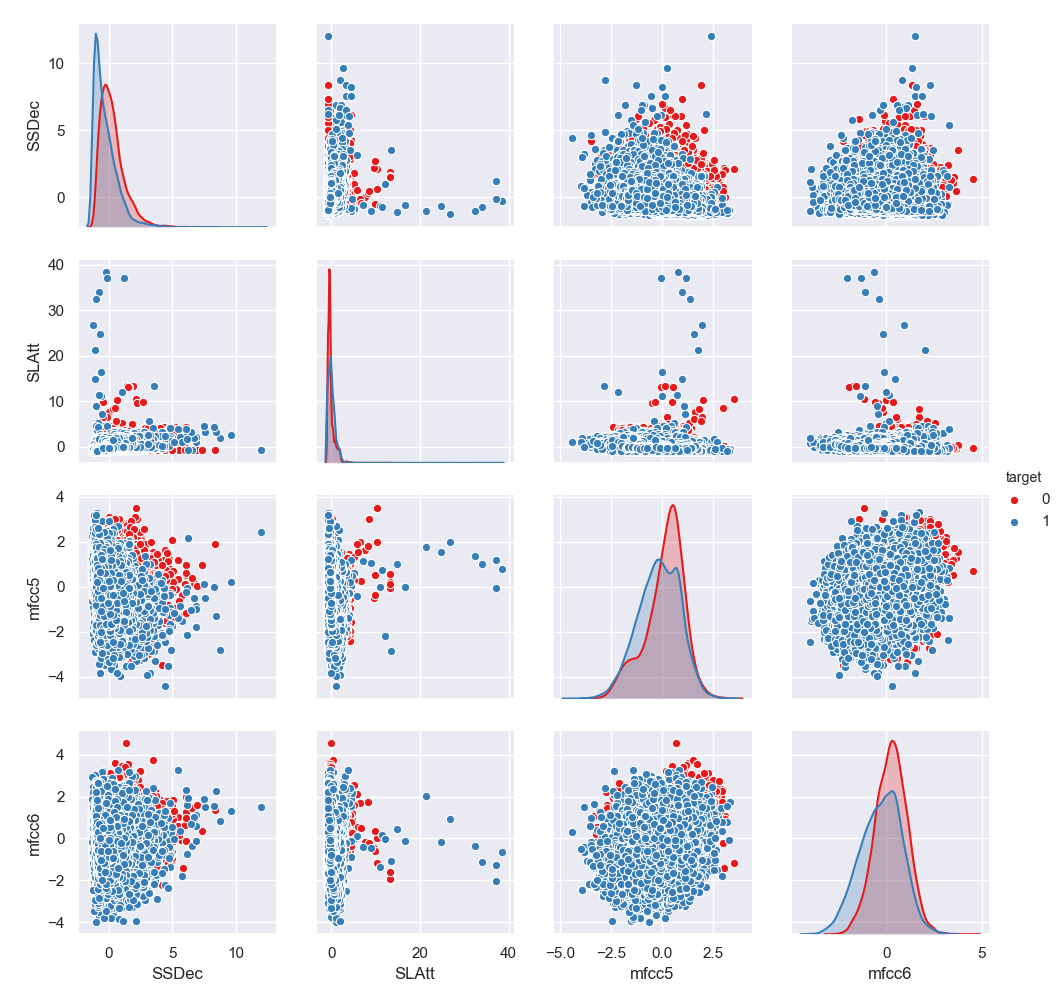
\includegraphics[width=0.7\textwidth]{res/figure_1.png}
\caption{Διαγράμματα συνδυασμών τεσσάρων χαρακτηριστικών ανά δύο}
\label{featureTable:table1}
\end{figure}
\begin{figure}[ht]
\centering
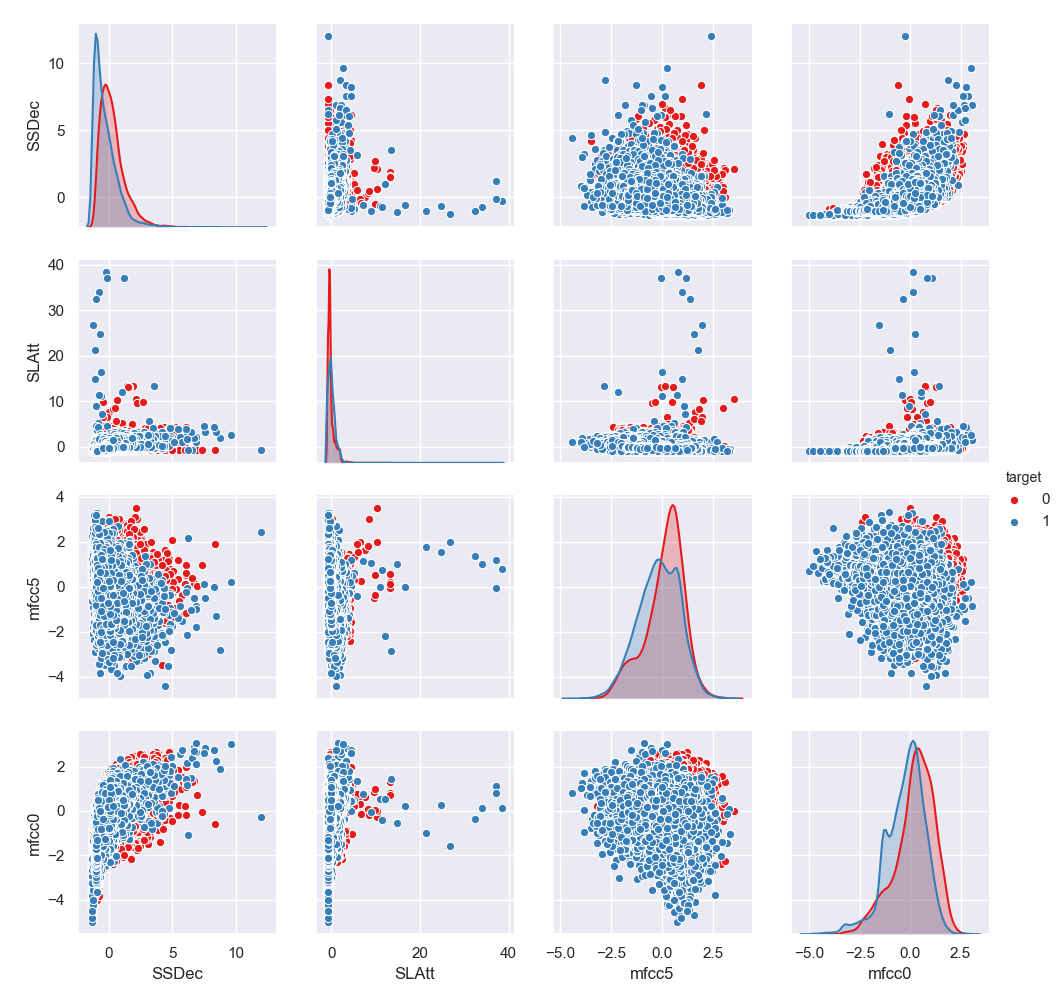
\includegraphics[width=0.7\textwidth]{res/figure_2.png}
\caption{Διαγράμματα συνδυασμών τεσσάρων χαρακτηριστικών ανά δύο}
\label{featureTable:table2}
\end{figure}

\section{Προεπεξεργασία δεδομένων}

Κατά την προεπεξεργασία των δεδομένων, δοκιμάστηκαν διάφορες τεχνικές έτσι ώστε να βρεθούν η βέλτιστη επιλογή χαρακτηριστικών και συνδυασμός μεθόδων. Οι μέθοδοι που δοκιμάστηκαν είναι η κλιμακοποίηση, κανονικοποίηση και ο συνδυασμός τους. Επίσης για την επιλογή των χαρακτηριστικών δοκιμάστηκαν το κατώφλι με βάση τη διακύμανση (VarianceThreshold) και η εκατοστιαία επιλογή (PercentileSelection), ενώ έγινε δοκιμή διάφορων τιμών των παραμέτρων αυτών των αλγορίθμων.

Τα αποτελέσματα παρουσιάζονται στον πίνακα \ref{table:tab}. Στην κλιμακοποίηση όλα τα χαρακτηριστικά έχουν μηδενικό μέσο και απόκλιση ίση με τη μονάδα ενώ στην κανονικοποίηση μετατοπίζονται οι τιμές τους ώστε να ανήκουν στο εύρος $[0,1]$. Τα VarianceThreshold και PercentileSelection, που είναι συναρτήσεις του sub-module feature\_selection της scikit-learn, αποκλείουν χαρακτηριστικά μέσω μετρικών αξιολόγησής τους. Στο VarianceThreshold, η μείωση του αριθμού των χαρακτηριστικών γίνεται με όρους διακύμανσης, δηλαδή αφαιρούνται όλα τα χαρακτηριστικά των οποίων η διακύμανση δεν ξεπερνά κάποιο κατώφλι, ενώ η PercentileSelection κατατάσσει τα χαρακτηριστικά με βάση τη διακριτική του ικανότητα και καταργεί όλα τα χαρακτηριστικά τα οποία βρίσκονται κάτω από ένα ποσοστό των καλύτερων καθορισμένο από το χρήστη.

\begin{table}[H]
	\centering
	\begin{tabular}{ l l l }
		\textbf{Μοντέλο} & \textbf{Μέθοδοι προεπεξεργασίας} & \textbf{Ακρίβεια} \\ \toprule
		 & Χωρίς προεπεξεργασία & 0.49 \\
		 & Scaling & 0.89 \\
		 & Κανονικοποίηση & 0.49 \\
		 & Scaling και κανονικοποίηση & 0.78 \\
		 & VarThreshold και scaling & 0.88 \\
		 & PercenSel και scaling & 0.81 \\
		 & VarThreshold, scaling και gamma=scale & 0.88 \\
		 & VarThreshold, scaling και sigmoid kernel & 0.58 \\
		\multirow{-9}{*}{SVM} & VarThreshold,  scaling και polynomial kernel (5\textsuperscript{ου} βαθμού) & 0.84 \\ \midrule
		Decision Tree & VarThreshold και scaling & 0.75 \\ \midrule
		Multi-Layer Perceptron & VarThreshold, scaling και rndState = 2 & 0.86 \\ \midrule
		Naive Bayes & VarThreshold και scaling & 0.65 \\ \bottomrule
	\end{tabular}
	\caption{Μέθοδοι προεπεξεργασίας για διάφορα μοντέλα. \small
	Εδώ για συντομία όπου VarThreshold εννοείται VarianceThreshold, PercenSel εννοείται PercentileSelection και scaling εννοείται κλιμακοποίηση.}
	\label{table:tab}
\end{table}

Εν τέλει, αποφασίστηκε να χρησιμοποιηθεί μόνο η κλιμακοποίηση, επειδή η κανονικοποίηση δεν είχε κανένα αποτέλεσμα και το κέρδος σε ταχύτητα ταξινόμησης των παραπάνω τρόπων μείωσης του αριθμού χαρακτηριστικών δεν ήταν αρκετό συγκριτικά με την μείωση της ακρίβειας ώστε να δικαιολογήσει τη χρήση τους στην υλοποίηση. Βοήθησαν παρ' όλα αυτά στον προσδιορισμό των χαρακτηριστικών που υπερτερούν.

Στη συνέχεια, σε μία προσπάθεια περαιτέρω κατανόησης και κατάταξης των χαρακτηριστικών με βάση τη διακριτική τους ικανότητα, απομονώθηκαν όλα και ελέγχθηκε η ακρίβειά τους ένα ένα. Τα αποτελέσματα έδειξαν ότι, τελικά, κανένα χαρακτηριστικό από μόνο του δεν είναι ικανό να δώσει ικανοποιητικό ποσοστό ακρίβειας. Ακόμα και αν πάρουμε το καλύτερο σε όρους ακρίβειας και το δοκιμάσουμε σε συνδυασμό με τα επόμενα καλύτερα, φαίνεται ότι η ακρίβεια αυξάνεται λίγο αλλά όχι αρκετά. Τέλος, αν επαναληφθεί ακόμα μία φορά η διαδικασία, φαίνεται ότι έχουμε και πάλι μια μικρή αύξηση στην ακρίβεια, η οποία όμως είναι αρκετά μακρυά από την ακρίβεια που επιτυγχάνεται χρησιμοποιώντας όλα τα χαρακτηριστικά.

\begin{table}[H]
	\centering
	\begin{tabular}{ l r r r }
		\textbf{Accuracy} & \textbf{Individually} & \textbf{With best first\textsuperscript{1}} & \textbf{With best second\textsuperscript{1}} \\ \toprule
		4Hz Mod & 0.58 & 0.66 & 0.73 \\
		Flat & 0.63 & 0.71 & 0.75 \\
		HFC & 0.58 & 0.65 & 0.72 \\ \midrule
		LAtt & 0.62 & 0.71 & 0.75 \\
		SC & 0.59 & 0.66 & 0.73 \\
		Scomp & 0.57 & 0.66 & 0.73 \\ \midrule
		SDec & 0.63 & 0.65 & 0.72 \\
		SEFlat & 0.51 & 0.65 & 0.72 \\
		SF & 0.55 & 0.69 & 0.75 \\ \midrule
		SFlat & 0.57 & 0.66 & 0.72 \\
		SLAtt & 0.63 & 0.71 & 0.74 \\
		SR & 0.60 & 0.66 & 0.72 \\ \midrule
		SSDec & \textbf{0.65} & - & - \\
		ZCR & 0.58 & 0.65 & 0.72 \\
		mfcc0 & 0.61 & 0.66 & 0.73 \\ \midrule
		mfcc1 & 0.58 & 0.67 & 0.73 \\
		mfcc2 & 0.52 & 0.66 & 0.73 \\
		mfcc3 & 0.56 & 0.69 & 0.76 \\ \midrule
		mfcc4 & 0.54 & 0.67 & 0.74 \\
		mfcc5 & 0.57 & 0.70 & 0.75 \\
		mfcc6 & 0.61 & \textbf{0.72} & - \\ \midrule
		mfcc7 & 0.57 & 0.68 & 0.75 \\
		mfcc8 & 0.55 & 0.67 & 0.74 \\
		mfcc9 & 0.54 & 0.67 & 0.73 \\ \midrule
		mfcc10 & 0.54 & 0.65 & 0.73 \\
		mfcc11 & 0.51 & 0.66 & 0.73 \\
		mfcc12 & 0.54 & 0.67 & 0.73 \\ \bottomrule
	\end{tabular}
	\caption{Ακρίβεια μεμονωμένων χαρακτηριστικών και συνδυασμών τους. \vspace{1em}\\\tiny
	1: όπου ``With best first'' εννοείται ο συνδυασμός του χαρακτηριστικού με το καλύτερο, ενώ ``With best second'' εννοείται ο συνδυασμός του χαρακτηριστικού με τον καλύτερο συνδυασμό που προέκυψε στο προηγούμενο βήμα}
\end{table}

Άρα, γίνεται προφανές ότι δεν υπάρχει κάποιο συγκεκριμένο, μοναδικό χαρακτηριστικό το οποίο ευθύνεται για το μεγαλύτερο ποσοστό της ακρίβειας του μοντέλου αλλά είναι ο συνδυασμός τους.

    \section{Machine Learning Models}

Στη συνέχεια αναφέρεται συνοπτικά η λειτουργία των μοντέλων που δοκιμάστηκαν για την εκπαίδευση των δεδομένων (οι ορισμοί είναι σύμφωνα με την ιστοσελίδα της analytics vidhya \footnote{https://www.analyticsvidhya.com/}) ενώ στο τέλος παρατίθεται ένας πίνακας στον οποίο φαίνονται οι διάφορες μέθοδοι και οι ακρίβειες που επιτεύχθηκαν.

\subsection{Support Vector Machine - SVM}

Τα SVMs ανήκουν στα μοντέλα επιβλεπόμενης μάθησης, και ο σκοπός τους είναι η εύρεση ενός γραμμικού υπερεπιπέδου (σύνορο απόφασης) το οποίο θα διαχωρίσει τα δεδομένα. Σε αυτόν τον αλγόριθμο, σχεδιάζουμε κάθε δεδομένο ως ένα σημείο σε έναν ν-διάστατο χώρο (όπου ν είναι ο αριθμός των features) με την τιμή κάθε feature να είναι η τιμή της εκάστοτε συντεταγμένης. Έπειτα, κατηγοριοποιούμε βρίσκοντας το υπερεπίπεδο το οποίο διαχωρίζει τις 2 κλάσεις καλύτερα.

\subsection{Decision Trees}

Τα δένδρα απόφασης ή decision trees ανήκουν στα μοντέλα επιβλεπόμενης μάθησης και εφαρμόζονται τόσο σε κατηγορικά όσο και συνεχή δεδομένα. Σε αυτόν τον αλγόριθμο, χωρίζουμε τα δείγματα σε πιο ομοιογενείς υποομάδες βασιζόμενοι στο χαρακτηριστικό που τα διαχωρίζει καλύτερα κάθε φορά.

\subsection{Multilayer Perceptron}

Ένα perceptron, μπορεί να κατανοηθεί ως οτιδήποτε δέχεται πολλαπλές εισόδους και παράγει μία έξοδο. Ο τρόπος όμως με τον οποίο συσχετίζεται η είσοδος την έξοδο εμφανίζει ενδιαφέρον. Αρχικά σε κάθε είσοδο ανατίθεται ένα βάρος, το οποίο εκφράζει τη σημασία της, ενώ στην έξοδο ένα κατώφλι. Τέλος, υπολογίζεται μία πόλωση η οποία μπορεί να θεωρηθεί ως το ποσό ευελιξίας του perceptron. Για λόγους απόδοσης, χρησιμοποιούνται πολλά perceptrons σε layers, τα οποία είναι πλήρως συνδεδεμένα μεταξύ τους.

\subsection{Naive Bayes}

Είναι μία τεχνική ταξινόμησης η οποία βασίζεται στο θεώρημα του Bayes με την υπόθεση ανεξαρτησίας ανάμεσα στους προβλέπτες. Με απλά λόγια, ο ταξινομητής Naive Bayes, υποθέτει ότι η ύπαρξη ενός συγκεκριμένου feature σε μια κλάση είναι ασυσχέτιστη με την υπάρξη οποιουδήποτε άλλου.

\subsection{Random Forest}

O Random Forest είναι ένας αλγόριθμος τύπου Bootstrap, με δένδρα απόφασης. Αυτό που πορσπαθεί να κάνει, είναι να φτιάξει δίαφορα δένδρα με διαφορετικά δείγματα και διαφορετικές αρχικές τιμές. Επαναλαμβάνει την διαδικασία και κάνει μια τελική πρόβλεψη για κάθε παρατήρηση, η οποία είναι συνάρτηση όλων των προβλέψεων.

\section{Αξιολόγηση μοντέλων}

Κατά την αξιολόγηση των μοντέλων, δοκιμάστηκε ποικιλία από τεχνικές εκπαίδευσης για τις διάφορες μεθόδους ταξινόμησης, μέχρι να βρεθεί ο βέλτιστος ταξινομητής. Μετά από πληθώρα δοκιμών, τα μοντέλα SVM και Random Forest αποδείχθηκαν τα καλύτερα στην ταξινόμηση, με βάση τη μετρική της ακρίβειας. Στον πίνακα \ref{table:tab1} φαίνεται η ακρίβεια των μοντέλων αυτών για διάφορους τρόπους εκπαίδευσης που δοκιμάστηκαν. Σε κάθε περίπτωση προηγήθηκε ανακάτεμα (shuffle) των εγγραφών του σετ δεδομένων.


\begin{table}[ht]
	\centering
	\begin{tabular}{@{} l p{9cm} r @{}}
		\toprule
		\textbf{Μοντέλο} & \textbf{Μέθοδος εκπαίδευσης} & \textbf{Ακρίβεια} \\ \midrule
		\multirow[m]{6}{*}{SVM} & Κλιμακοποίηση και τυχαίο split & 0.94 \\
		 & Κλιμακοποίηση και 5-fold cross validation & \textbf{0.96} \\
		 & Κλιμακοποίηση, PCA (μείωση σε 10 χαρακτηριστικά) και τυχαίο split & 0.92 \\
		 & Κλιμακοποίηση, PCA (μείωση σε 10 χαρακτηριστικά) και 5-fold cross validation & 0.93 \\ \midrule
		\multirow[m]{3}{*}{Random Forest} & Κλιμακοποίηση και 5-fold cross validation & 0.95 \\
		 & Κλιμακοποίηση, PCA (μείωση σε 10 χαρακτηριστικά) και 5-fold cross validation & 0.94 \\ \bottomrule
	\end{tabular}
	\caption{Ακρίβεια των δύο καλύτερων μοντέλων (SVM και Random Forest) για διάφορες μεθόδους εκπαίδευσης. \small
	Όπου χρησιμοποιήθηκε cross validation κρατήθηκε η ακρίβεια του καλύτερου fold.}
	\label{table:tab1}
\end{table}

Η μέγιστη ακρίβεια που επιτυγχάνεται είναι 96\% με κλιμακοποίηση και 5-fold cross validation χρησιμοποιώντας SVM μοντέλο με γκαουσιανό (Radial Basis Function ή RBF) πυρήνα.

\section{Συμπεράσματα}

Παρατίθεται στη συνέχεια ο πίνακας στον οποίο φαίνεται η μέγιστη ακρίβεια που επιτεύχθηκε για κάθε μοντέλο που δοκιμάστηκε.

\begin{table}[h]
	\centering
	\begin{tabular}{@{} l r @{}}
		\toprule
		\textbf{Method} & \textbf{Αccuracy}\\\midrule
		SVM & \textbf{96.06}   \\
		Decision Tree & 86.51 \\
		MultiLayer Perceptron & 90.34 \\
		Naive Bayes & 70.25 \\
		Random Forest & 95.49 \\
		SVM (PCA(10)) & 90.02 \\ \bottomrule
	\end{tabular}
	\caption{Ακρίβεια μοντέλων ταξινομητών που δοκιμάστηκαν}
\end{table}

Όπως φαίνεται, τα Support Vector Machines και ο αλγόριθμος Random Forest αποδίδουν τα καλύτερα αποτελέσματα με 96\% και 95\% ακρίβεια αντίστοιχα, ενώ αρκετά καλά αποδίδουν και τα Multilayer perceptrons. Παράλληλα, βλέπουμε ότι τα χειρότερα αποτελέσματα στη ταξινόμηση δίνει ο Naive Bayes με περίπου 70\% ακρίβεια. Τέλος, η εφαρμογή του PCA είναι φανερό ότι μείωσε αρκετά την ακρίβεια των μοντέλων και για αυτόν τον λόγο συνίσταται μόνο στην περίπτωση που υπάρχει κάποιος σοβαρός χρονικός περιορισμός κατά την ταξινόμηση καθώς, λόγω της μείωσης των χαρακτηριστικών από 27 σε 10, αυτή θα εκτελείται πιο γρήγορα.


    \bibliographystyle{ieeetr}
    \bibliography{cites}{}
\end{document}